\documentclass[uplatex,dvipdfmx]{jsarticle}

\usepackage[uplatex,deluxe]{otf} 
\usepackage[noalphabet]{pxchfon} 
\usepackage{stix2} 
\usepackage[fleqn,tbtags]{mathtools} 
\usepackage{amsmath}
\usepackage{url}
\usepackage{float} 

\setcounter{tocdepth}{3}
\usepackage{moreverb}
\usepackage{lscape}
\usepackage{ascmac}
\usepackage{xurl}
\usepackage{graphicx} % 画像挿入用

\begin{document}

\title{危険交差点警告システム}
\author{25G1051 近藤巧望}
\maketitle

\section{はじめに}

\subsection{社会的背景}
自転車は温室効果ガスを排出しない移動手段であり,環境に優しい交通手段として注目されている.
日本の自転車保有台数は約6870万台(つまり約二人に1台)となっており,交通渋滞の緩和や健康促進,
地球温暖化等の環境問題への配慮の観点から,政府も自転車活用推進法に基づき自転車の利用を推奨している
\cite{ref:koutuusyou_1,ref:koutuusyou_2}.

しかし交通事故に焦点を当てると,自転車利用中の出会い頭衝突事故は2023年時点で全体の52.9\%と,
自転車事故の中で最も多く発生している事故であり,深刻な問題となっている\cite{ref:sonpo_1}.
自転車事故は特に交差点で発生することが多く,視界が遮られたり信号の認識が困難だったりするため,事故が起こりやすい.

従来の交通事故対策として交通安全教育や,道路交通法といった法規制がある.
しかし,これらの対策だけでは,利用者の多様な判断・行動パターンや道路上での様々な危険的要因に十分に適応し,事故の発生を根本的に解決することは困難である.
例えば,交通安全教育は安全意識の向上に寄与するが,交通安全教育では即時性がなく交通ルールなどの知識が形骸化してしまうことから,
すべての自転車利用者が常に高い安全意識を持って行動することが保証できない.
法規制の強化についても利用者の行動変容を促すには限界があり,瞬間的な判断が求められる交差点での事故防止には,
さらに直接的かつ即時的な対策が必要である.

以上のことから,従来の交通安全教育や法規制に加えて,技術的な新しい事故防止策が求められる.
特に,リアルタイムで危険を検知し利用者に警告するようなシステムは個々の利用者の安全意識に依存せず客観的な危険情報を提供することで,
従来の交通安全教育や法規制の限界を補完するという形で事故率を低減させる可能性をもっている.

\subsection{問題点}
既存のリアルタイム危険検知システムとして,自動車向けのナビゲーションで事故多発エリアを警告する仕組みがある.
このシステムは,GNSS(Global Navigation Satellite System)で位置情報を取得し,地図データおよび事故多発エリアのデータベースと照合することで,
特定の範囲に進入した際に音声警告を行うものである.

しかし,この方式にはデータ依存性による検知精度の限界という技術的問題がある.
警告判定は過去の事故発生地点をもとにしたデータベース検索により行われるため,
データの空間的偏り(都市部と地方でのデータ量差)や,時間的遅延(道路工事や交通環境変化への更新遅れ)により,
リアルタイム性と正確性が確保できない.
特に,自転車のように走行範囲が狭く道路環境の変化が激しい場合,この更新遅れは致命的な影響を及ぼす.

この問題を解決するために,事故データに依存せずに危険な交差点を検出できる仕組みとして,AI(Artificial Intelligence)を用いた画像認識技術を導入する手法を検討した.
しかし,この手法にも新たな技術的課題が存在する.
航空画像から交差点や障害物を自動判定するためには高精度な学習済みモデルが必要であり,
照明条件や建物,街路樹などの外的要因によって認識精度が変動する.
また,AI処理は大量の行列演算を伴うため,リアルタイム処理時には計算負荷や電力消費が増大し,スマートフォン上での長時間動作には不向きである.

\subsection{目的}
本提案の目的は,自転車での出会い頭衝突を防止し,交通事故による負傷者および死者数を減少させることである.
具体的には,出会い頭衝突による事故件数を現状から約10%削減することを目標とする.
令和6年中の自転車関連事故全体の件数は67,531件であり,そのうち52.9%にあたる約35,700件が出会い頭衝突であることから,
本提案により約3,570件の事故削減が期待できる.

この10\%という目標値は,既存の自動車向け衝突防止支援システムADAS(Advanced Driver-Assistance Systems)が,
衝突事故を約10\%削減したとする先行研究の成果を基準として設定したものである\cite{ref:adas_purpose}.
ただし,同研究ではデータ数の不足により統計的有意差が得られなかったため,
本提案ではより実用的な環境(自転車交通)において,この削減効果を再現・拡張することを目的とする.

さらに,前節で述べたような技術的課題である「事故データに依存した検知精度の限界」および
「画像認識による処理負荷・電力消費の問題」を克服するために,
本提案では,事故データベースと画像認識を状況に応じて切り替えて利用するハイブリッド型危険検知アルゴリズムを提案する.
この手法では,事故データが十分に存在する地域ではデータベースを用いて高速かつ低電力で危険検知を行い,
事故データが不足している地域では航空画像を用いたAI画像認識に切り替えることで,
検知精度とリアルタイム性の両立を実現する.

これにより,既存システムの問題であった「偏った事故データへの依存」や「環境変化への追従遅れ」を改善し,
地域差の少ない包括的な危険検知を可能にする.
本提案システムを導入することで,より広範囲での自転車走行安全を確保し,
子どもから高齢者まで幅広い層の自転車利用者が安心して走行できる社会の実現に貢献することを目指す.

\section{解決策としての提案手法}

\subsection{提案手法の概要}
本提案は,アプリケーションとして導入し,スマートフォンと連携することで,ユーザーに対してリアルタイムで危険警告を提供する.
危険の判定処理方法として,画像認識技術による交差点の危険検知と,事故データベースによる危険検知の2つの手法を用いるため,
状況に応じて切り替えられるアルゴリズムを提案する.

画像認識での判定では,まずGNSSを用いて利用者の位置情報を取得する.この際,GNSSにはGPSとQZSSを併用することで,正確な位置情報を取得できるようにする.
次に,その位置情報をもとにGoogle Maps Static APIを用いて現在地周辺の道路の航空画像を取得し,事前に学習させたAIによる画像認識技術を用いて交差点を検出する.
危険が検出された場合には,利用者に音声とバイブレーションで警告を行う.
使用時は,スマートフォンにアプリケーションをインストールし,GNSS機能を有効にした状態でアプリケーションを起動し,固定具で自転車のハンドルに取り付けて利用する.

事故データベースでの判定ではまず,警察庁や自治体が公開している事故データベースから,座標と事故件数のデータを取得し,
一定の半径内を「事故多発エリア」として設定する.その後GNSS(GPS+QZSS)で利用者の緯度経度を取得し,現在位置から一定半径内の事故件数を検索する.
事故件数に基づいて危険度スコアを算出し,閾値を超えた場合に警告を発する.

2つの手法を切り替えるアルゴリズムについても説明する.
前提として,常時入力としてGNSSでの位置座標と事故データベースをしている.
主に事故データの活用をベースとし,事故データが十分に存在する地域では事故データベースを用いて危険検知を行う.
一方で事故データの数が閾値以下の場合に,画像認識による危険検知を行う.どちらも危険が検出されなかった場合は,次の位置情報の取得まで待機する.

\subsection{提案手法の構成要素について}

\begin{table}[H]
  \centering
  \caption{システムの構成要素}
  \label{tab:system_components}
  \begin{tabular}{|c|l|l|}
    \hline
    項目 & 構成要素 & 備考\\ \hline
    1 & スマートフォンGNSS & 位置情報を取得するためのGNSS機能(GPSとQZSSを使用) \\ \hline
    2 & 事故データベース & 警察庁や自治体の公開事故データを活用した危険度判定 \\ \hline
    3 & Google Maps Static API & 現在地周辺の航空画像を取得 \\ \hline
    4 & 画像認識モデル & 画像の分類・危険な交差点を検出 \\ \hline
    5 & 切り替えアルゴリズム & 事故データと画像認識を状況に応じて使い分け \\ \hline
  6 & 警告システム & 利用者に音声とバイブレーションで警告を行う \\ \hline
  \end{tabular}
\end{table}

\begin{figure}[H]
  \centering
  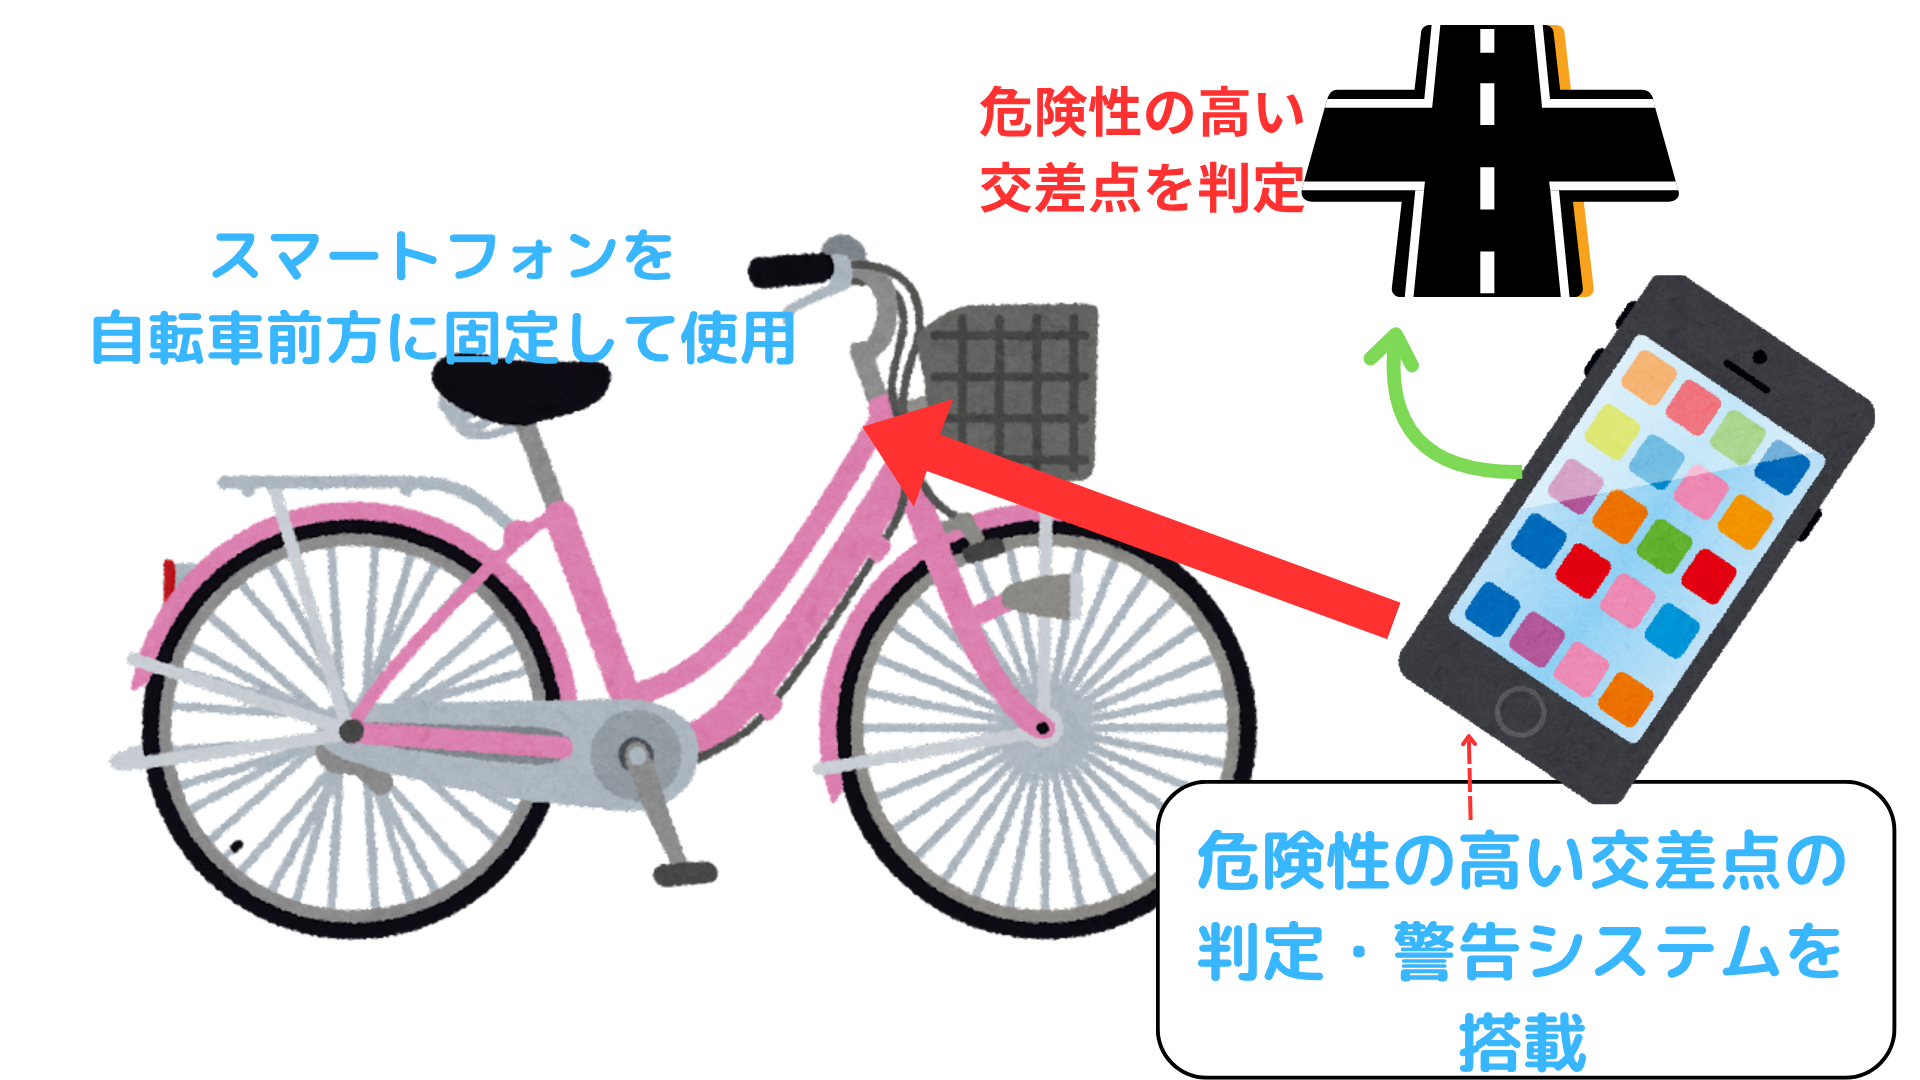
\includegraphics[width=0.8\textwidth]{./Figs/gainenzu_final.png}
  \caption{システムの概念図}
  \label{fig:system_final}
\end{figure}

システムの構成要素を表\ref{tab:system_components}に,システムの概念図を図\ref{fig:system_final}に示す.
本システムは主に6つの要素から構成される.

まず,利用者の位置情報を取得するためのGNSSである.
本提案では,QZSSとGPSを併用するが,QZSSとは日本国内で運用されている衛星測位システムであり,主に日本とアジア太平洋地域の任意の地点で正確な位置情報を,人工衛星からスマートフォンで受け取ることができる.
スマートフォンの内部にはGPS(Global Positioning System)とQZSSに対応したGNSS受信モジュールが搭載されているため,GPSだけでは不十分な点を補う形でQZSSを併用することで,より正確な位置情報を取得できる.
GPSのみの使用に限定してしまうと,都市部のビル街や山間部で衛星が遮蔽されやすく補足数が減るのに加え,マルチパスによって誤差が大きくなる可能性がある.
対してQZSSは,GPSと比べて日本国内での測位精度が高いことが知られている他,
QZSSは日本の天頂付近を通過するように設計されているため,都市部の高層ビル街や山間部などでの受信性能が向上するという利点がある\cite{ref:qzss}.
しかし,衛星数が2025年時点で4機と少なく,単独での測位には限界があるため,GPSと併用することで,より安定した位置情報の取得が可能になる.
以上の理由から,本提案ではGPSとQZSSを併用することにした.
これらのGNSSを用いることで,利用者の正確な位置情報をリアルタイムで取得することができ,
利用者の位置情報は,航空画像の取得範囲を特定したり,事故データベースの検索範囲を特定するために使われる.

次に,危険判定の指標となる事故データベースである.
これは,警察庁や自治体が公開している交通事故の発生地点や件数を座標情報として集積したものである.
このデータベースには,過去数年間の交通事故が位置情報とともに記録されており,特に交差点やその周辺での事故件数が多い場所を
「事故多発エリア」として抽出できる.
本提案では,GNSSによって取得した利用者の位置情報を基準とし,一定の半径以内に記録されている事故件数を検索する.
その結果を基に,件数が多いほど危険度が高いと判定する危険度スコアを算出し,一定件数以上の事故が登録されている場合に警告を行う.

画像認識手法では,Google Maps Static APIを用いて利用者の周辺の交差点情報を取得する.
Google Maps Static API とは,Google が提供する地図画像を取得するための API(Application Programming Interface) であり,
航空写真や地図画像を取得することができる.
Google Maps Static APIは,URLにパラメータを指定するだけで簡単に地図画像を取得できるうえに使用するための料金に無料枠があることから,
扱いやすさとコスト面で優れている.
また,ドキュメントが豊富で導入が容易であることも採用理由の一つである.
同じく地図を表示させるAPIとしてGoogle Maps JavaScript APIがあるが,Google Maps Static APIはデータの読み込み量が少ないという点でも優れている.
Google Chromeのデベロッパー ツールを用いてGoogle Maps Static APIとGoogle Maps JavaScript API双方の公式サンプルページにおけるデータ転送量を確認したところ,
Google Maps Static APIはデータの読み込み量が63.8 kB,Google Maps JavaScript APIはデータの読み込み量が433 kBであり,
約7倍の差があった\cite{ref:developer_static,ref:developer_js}.Google Maps Static APIは静的な画像を取得するのに対し,Google Maps JavaScript APIは動的に地図を表示するため,
ほぼ単一な画像サイズと同じデータ量であるGoogle Maps Static APIの方が,地図表示プログラム一式を読み込むGoogle Maps JavaScript APIよりもデータの読み込み量が少なくなり,
通信速度が高速である.
本システムは高速なリアルタイム処理が求められるため,データの読み込み量が少ないGoogle Maps Static APIがより適している.

画像認識モデルは,機械学習により画像から危険な交差点を検出する.
道路の形状から交差点を判定し,さらに形状・塀・街路樹などの障害物から危険度を分類する.
危険度によって道路を分類することで,すべての交差点に近づくたびに作動することを防ぎ,必要な場合のみ警告を行う.

警告の作動タイミングについては,交差点の手前約30mで警告を行う.
利用者が警告に気づいてからブレーキをかけるまでの距離(以下,空走距離)は,一般的な自転車の移動速度時速約15km(秒速約4.2m)を加味し,
利用者が警告を受けてから行動に移すまでの時間を少し余裕を見て1.5秒と仮定する\cite{ref:bycicle, ref:responsibility}.
これにより,空走距離は式\eqref{eq:reaction_time}のように計算できる.
\begin{align}\label{eq:reaction_time}
4.2\,\mathrm{m/s} \times 1.5\,\mathrm{s} = 6.3\,\mathrm{m}
\end{align}
さらに,ブレーキをかけてから完全に止まるまでの距離(以下,制動距離)はgを重力加速度,μを摩擦係数として,(2)式のように計算できるため,
平坦な乾いた道路での摩擦係数μを0.7,重力加速度gを9.8m/s\textsuperscript{2}とすると,制動距離は(3)式のように計算できる\cite{ref:brake_distance,ref:dry_road}.
\begin{align}
  制動距離S = \frac{初速度の二乗}{2g\mu}
\end{align}
\begin{align}
    S = \frac{(4.2)^2}{2\times9.8\times0.7} \approx 1.3\,\mathrm{m}
\end{align}
したがって,利用者が完全に停止するために最低限必要な距離は,空走距離と制動距離を合わせて,6.3m+1.3m=7.6mとなる.
しかし,これは急ブレーキをかけた場合に止まれる最低限の距離であり,本当に減速するべきかという状況判断や,落ち着いて減速・停止するという心理的余裕,さらに雨などで路面が濡れているといった悪条件を考慮すると,
最低停止距離7.6mと同等かそれ以上の余裕を確保する必要がある.
さらに,上記の計算は平均的な自転車の速度を基にしているため,より速い速度で走行している場合には,より長い距離が必要になるうえ,
AIの認識に時間がかかる可能性もある.
そのため,最低停止距離を約2倍した数値よりもさらに余裕を持った距離として,交差点の約30m手前で警告を行うこととした.

切り替えアルゴリズムについては,事故データベースを主軸とし,事故データが十分に存在する地域では事故データベースを用いて危険検知を行う.
一方で事故データの数が閾値以下の場合に,画像認識による危険検知を行う.
どちらも危険が検出されなかった場合は,次の位置情報の取得まで待機する.
事故データベースを主軸とする理由として,事故データベースは位置情報さえあれば,画像認識のように画像を取得する必要がなく,AIの処理も不要であるため,電力消費と処理速度の問題を軽減できるからである.
また,事故データベースは過去の事故データに基づいているため,画像認識よりも安定した性能が期待できる.
一方で,事故データが不足している地域では,画像認識を用いることで,事故データに依存しない柔軟な危険検知が可能になる.
このように,事故データベースと画像認識を状況に応じて使い分けることで,両者の利点を活かしつつ,欠点を補完することができる.

警告システムは危険性の高い交差点が検出された場合,音声とバイブレーションで警告を行う.
光での警告では,明るい時間帯では気が付かない可能性があることや,周囲の状況によって視認性が低下するため,
警告の伝わりやすさと安全性を考慮して,音声とバイブレーションでの警告を採用した.

開発言語としては,iOS向けにはSwift/Objective-C,Android向けにはKotlin/Javaを用い,共通の画像認識エンジン部分にはPythonで開発したモデルをTensorFlow Lite やPyTorch
Mobileなどのフレームワークで変換・最適化して組み込む.

アプリケーションとしての運用には,スマートフォンのバッテリーについても懸念がある.
QZSSの常時利用,航空画像のダウンロード,画像認識モデルのリアルタイム推論は電力を消費するためシミュレーションの結果,連続使用で1時間あたり約15-20\%のバッテリー消費が見込まれる.
つまり,通勤や通学などで片道30分程度の利用を想定すると,往復で1時間程度の使用で約15-20\%のバッテリー消費が見込まれるため,日常的な使用には十分対応できると考えられる.
このバッテリー消費をさらに抑えるために,自転車の速度などに応じて不要な処理を中断することや,スマートフォン内の低消費電力モードを活用することによって,バッテリー消費を最小限に抑える工夫を行う.

\subsection{AIの学習方法}
画像認識モデルの学習方法について説明する.
学習データとしては,様々な地域での道路の航空画像を収集し,それらの画像に対して,交差点か否か・交差点の危険度をラベル付けする.
この際,交差点の画像のみでなく,交差点ではない道路の画像も収集することで,AIモデルが交差点と非交差点を正確に識別できるようにする.
学習のために用意する航空画像のデータセットの規模は,例えば5万枚程度の比較的小規模なものとして初期段階で用意していく.
その後には,より複雑な状況にも対応できるように,年間約1万枚のデータを継続的に追加収集していく.

交差点の危険度については,道路の交差パターン,停止線,交通標識の有無,周囲の建物や植生による視界の遮蔽度合いといった複合的な視覚情報を考慮して,「非交差点」「安全な交差点」「危険な交差点」の3段階に分類する.
このようにして収集したデータを用いて,画像認識モデルを作成する.道路の形状においては,十字路や五差路といった複雑な形状も考慮する.

本システムでは,画像認識技術として畳み込みニューラルネットワーク(CNN:Convolutional Neural Network)を採用する.
畳み込みニューラルネットワークは,画像の特徴を自動的に学習する深層学習手法であり,特に画像分類や物体検出において一般的に用いられる\cite{ref:newral}.

本システムが目指すリアルタイム警告には高い認識精度が求められる.
CNNと同じく画像認識に用いられる手法として,近年注目されているViT(Vision Transformer)があるが,
ViTは事前学習に大規模なデータセットが必要なのに対して,CNNは比較的小規模なデータセットでも高い精度を達成できることが報告されている.
先行研究では小規模データセットにおいて,CNNの一種であるDenseNet-BC(k=40),ResNeXt-29(8×64d),Res2NeXt-29(6c×24w×6s-SE)の精度がそれぞれ
82.82\%,82.23\%,83.44\%であり,ViTの一種であるDeiT-T,DeiT-S,PVT-Tはそれぞれ
67.59\%,66.55\%,69.62\%と,ViTよりもCNNの精度が高いことが示されている\cite{ref:cnn_vit}.
以上の理由から、本システムでは実績の豊富なCNNアーキテクチャを採用することにした。

交差点危険度分類においては,畳み込みニューラルネットワークが道路の形状パターン,障害物の配置,交通環境などの複雑な視覚的特徴を学習し,
これらの特徴から交差点の危険度を自動的に判定する.
従来の画像処理手法と比較して,畳み込みニューラルネットワークは大量の学習データから自動的に特徴を抽出できるため,
より高精度で汎用性の高い交差点認識が可能となる.

\subsection{システム動作フロー}
\subsubsection{切り替えアルゴリズムについて}
\begin{figure}[H]
  \centering
  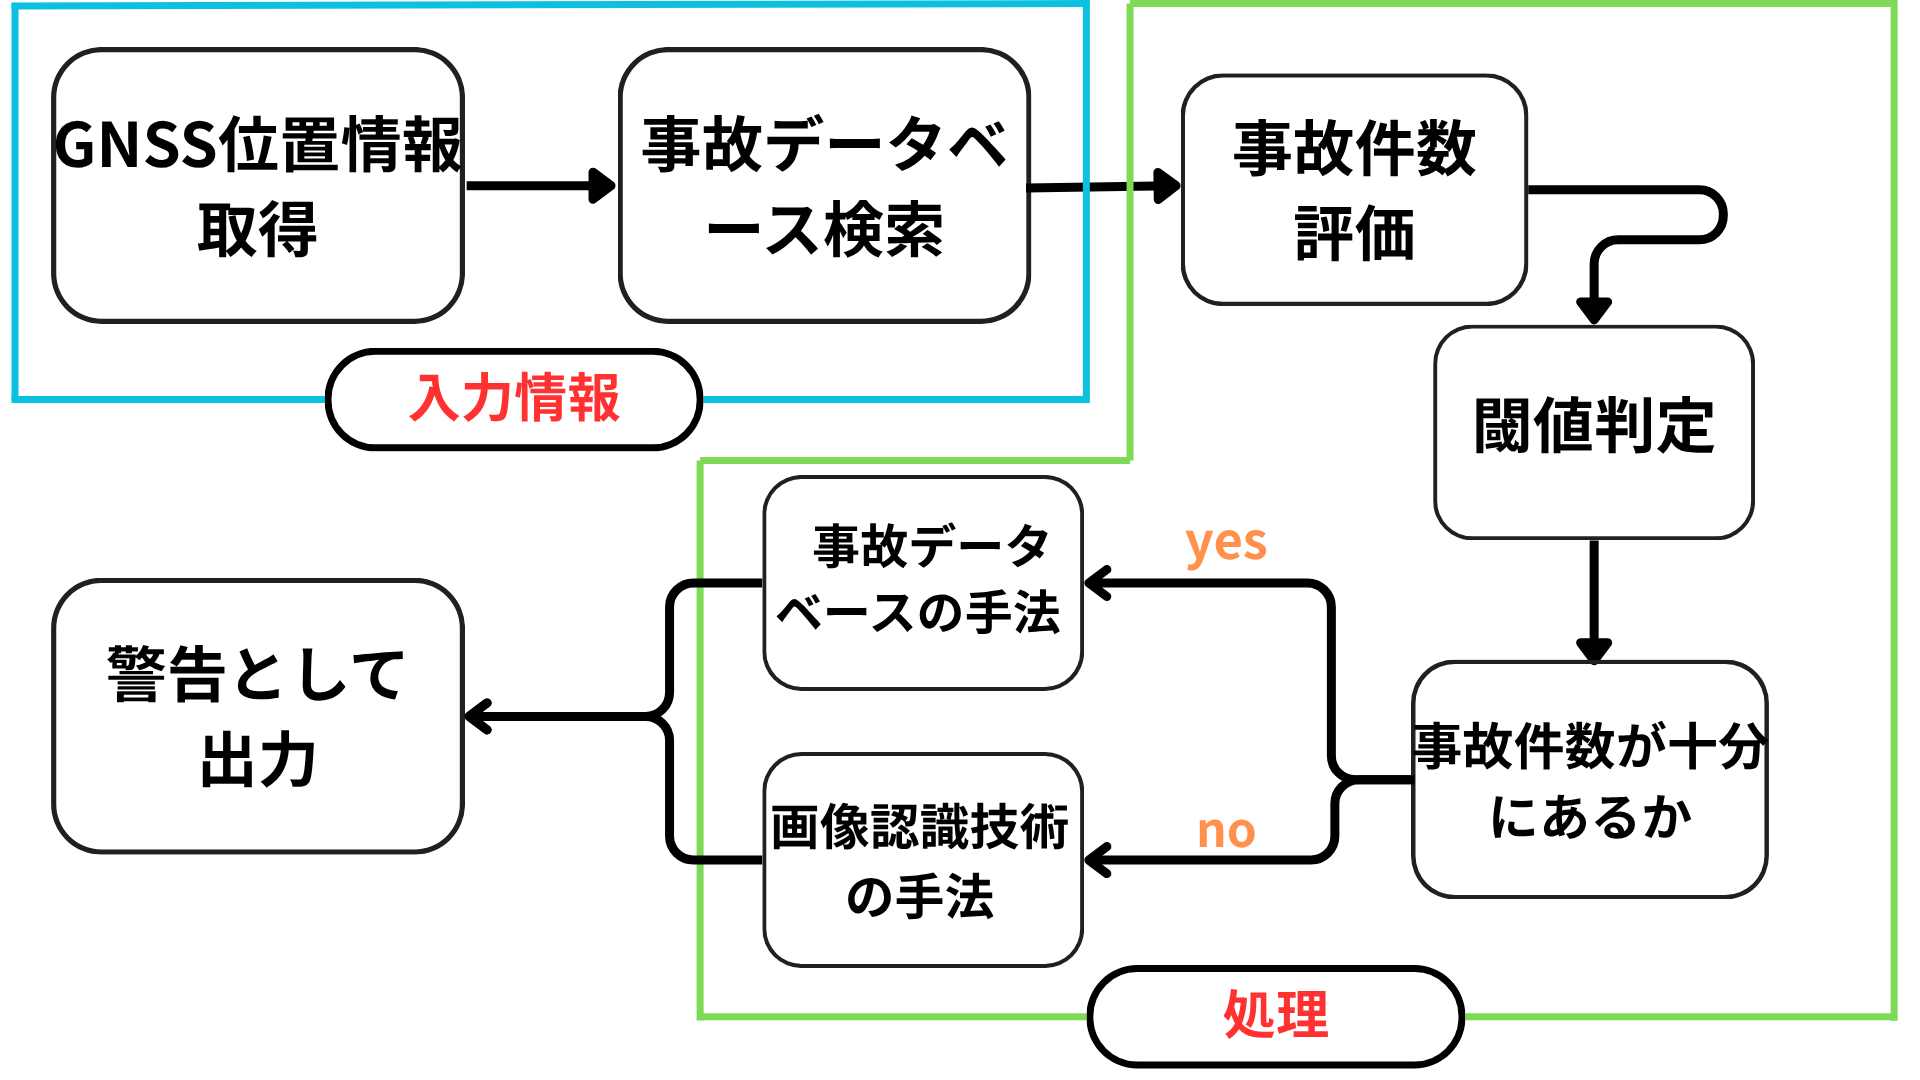
\includegraphics[width=12cm]{./Figs/system_all.png}
  \caption{切り替えアルゴリズムのシステム構成図}
  \label{fig:system_all}
\end{figure}

危険検知の手法を切り替えるアルゴリズムのシステム構成図を図\ref{fig:system_all}に示す.
本システムは,事故データベースを用いた判定法と,航空画像を用いた画像認識判定法を状況に応じて切り替えるアルゴリズムによって構成される.

切り替えアルゴリズムについて説明する.
本アルゴリズムでは,まずGNSSにより利用者の現在位置を取得し,
この位置情報を基に,中心点を利用者の座標とする半径$50$mの範囲内に記録されている事故件数を
事故データベースから検索する.
得られた事故件数があらかじめ設定した閾値以上であれば,事故データベースに基づく判定を行う.
一方で,件数が閾値を下回る場合は,航空画像を取得し,画像認識による判定に切り替える.
生活道路における交通事故についての先行研究では,事故件数の閾値を3件に設定した結果,
交通事故全体の約84\%をカバーできたと報告されている\cite{ref:accident_spot}.
また,一般的に1〜2件程度では統計的な偏りが大きいため,信頼できるデータとみなすには3件以上が妥当である.
したがって,閾値を3件に設定することが適切であると考えられる.

\subsubsection{事故データベースによる判定方法について}
\begin{figure}[H]
  \centering
  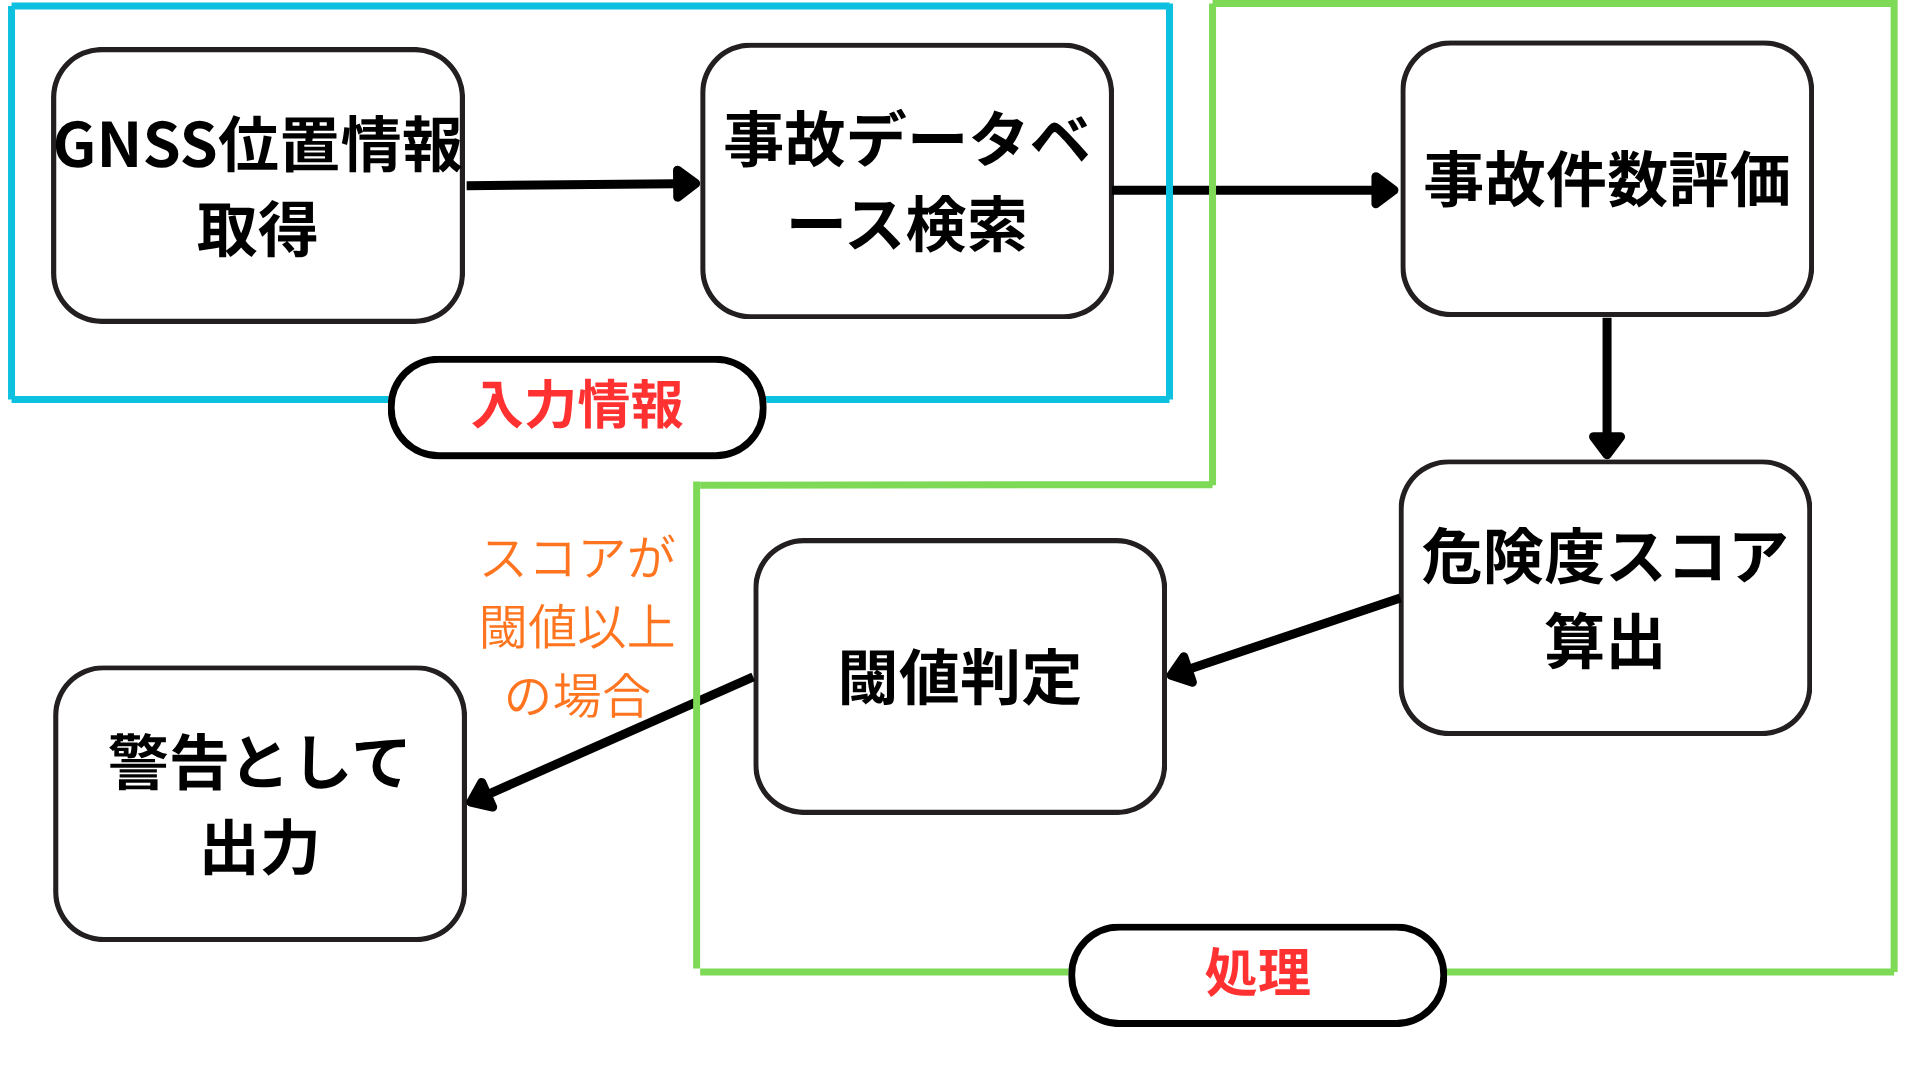
\includegraphics[width=14cm]{./Figs/system_data.png}
  \caption{事故データベース判定のシステム構成図}
  \label{fig:system_data}
\end{figure}

事故データベースを参照する判定方法のシステム構成図を図\ref{fig:system_data}に示す.
事故データベースによる判定方法は,切り替えアルゴリズムにおいて,事故データが十分に存在すると判断された地域で用いられる.

事故データベースを用いた危険判定手法について述べる.
本手法は,警察庁や自治体が公開している交通事故統計データを基に作成した事故データベースを利用し,
利用者の現在位置の周囲における過去の事故発生状況をもとに危険度を推定するものである.
この方法は,事故データが十分に蓄積された地域において有効であり,AI画像認識などの高負荷な処理を行うことなく,
低消費電力かつ高速に危険検知を行うことができる.

まず,スマートフォンに内蔵されたGNSS(GPSおよびQZSS)によって利用者の現在位置を取得する.
取得した位置情報を基に,事故データベースから半径50 m以内の範囲に記録されている事故データを検索する.
このデータベースには,警察庁や自治体が公開する交通事故統計をもとに,事故の発生地点(緯度・経度),発生日時,
事故形態(出会い頭・追突・右折巻き込みなど),交通主体(自転車・自動車・歩行者)および被害程度(死傷・物損)が登録されている.
検索範囲内に存在する事故件数を$N$とし,この値を基に危険度スコア$S_d$を算出する.
危険度スコアは,データベース全体における最大事故件数$N_{max}$を基準に次式で求められる.
\begin{align}
  S_d = \frac{N}{N_{max}}
\end{align}
算出した$S_d$が事前に設定した閾値$S_{th}$以上(本提案では3以上)である場合,その地域を「事故多発地域」と判定し,利用者に対して警告を出力する.
警告はスマートフォンの音声およびバイブレーション機能によって行われ,
「この先、事故の多い交差点があります。注意してください。」といったメッセージを音声で出力するとともに,
触覚的な振動により注意喚起を促す.

画像認識による判定方法との相違点としては,事故データベースを用いることで,過去の実際の事故情報に基づくため,信頼性の高い危険判定が可能である点が挙げられる.
さらに,AI画像認識を用いる場合と比較して演算負荷が小さく,通信量や電力消費を大幅に抑えることができる.
一方で,事故データが十分に蓄積されていない地域や,道路形状が変更された新設地域では,適切な危険評価が行えないという課題も存在する.
そのため,この手法単独ではカバーしきれない状況を補うために,次節で述べる画像認識による判定方法を組み合わせ,
事故データが不足している地域では自動的に画像認識判定に切り替える構成としている.

\subsubsection{画像認識による判定方法について}
\begin{figure}[H]
  \centering
  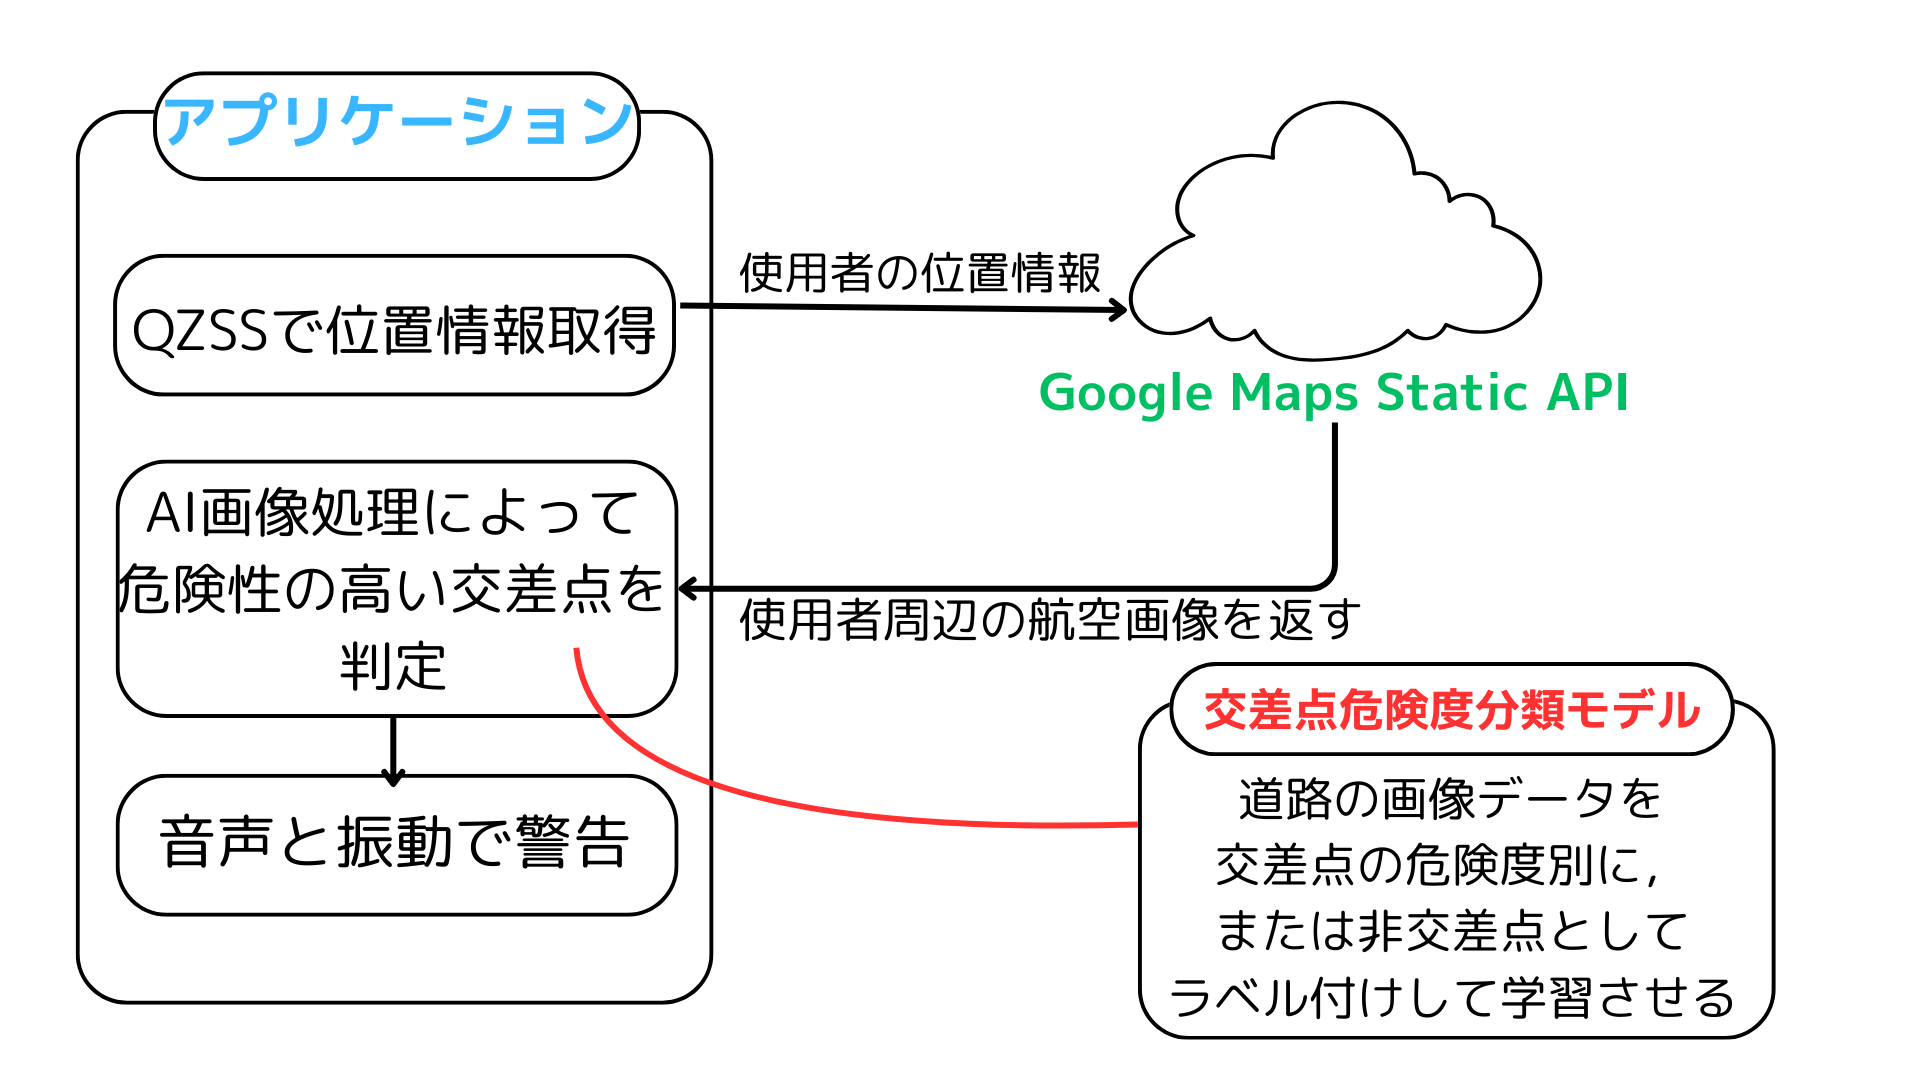
\includegraphics[width=14cm]{./Figs/system_new.png}
  \caption{画像認識判定のシステム構成図}
  \label{fig:system_new}
\end{figure}

本システムの動作の流れを図\ref{fig:system_new}に示す.
画像認識による判定方法は,切り替えアルゴリズムにおいて,事故データが不足していると判断された地域で用いられる.

まず,スマートフォンのGNSSから位置情報を取得する.
次に,Google Maps Static APIを用いて,現在地周辺の航空画像を取得する.
取得した航空画像は,事前に学習させた畳み込みニューラルネットワークによって処理され,道路の形状や障害物の配置などを解析し,交差点の有無と危険度を自動判定する.
危険性の高い交差点が検出された場合,利用者に対して音声とバイブレーションで警告される.
具体的には,スマートフォンから「危険な交差点があります.注意してください」といった警告が行われるとともに,
バイブレーション機能を用いて触覚的な警告も同時に行われる.

事故データベースによる判定方法との相違点としては,画像認識による判定では航空画像の取得とAI処理が必要になるため,処理時間と電力消費が増加することが挙げられる.
一方で,事故データベースに依存しないため,事故データが不足している地域や新たに開発された道路でも危険検知が可能である.
また,画像認識は道路の物理的な特徴(見通しの悪さ,障害物の配置など)をリアルタイムで評価できるため,道路改良後の状況変化にも即座に対応できるという利点がある.
このように,両手法はそれぞれ異なる特徴を持ち,状況に応じて使い分けることで,より包括的な危険検知システムを実現できる.

\section{提案手法の実現可能性の評価と妥当性の検証}

\subsection{主張・手法のまとめ}
本提案は,自転車利用者の注意力の限界を補い,出会い頭衝突の事故を防ぐための危険交差点警告システムである.
既存技術の問題点として,事故データベースに依存する手法は事故データが不足している地域での対応が困難であり,
画像認識に依存する手法は処理負荷が高く,リアルタイム性と電力消費の面で課題があることを指摘した.
これらの問題を解決するために本システムでは,事故データベースによる危険検知と画像認識による危険検知の2つの手法を状況に応じて切り替えるハイブリッドアルゴリズムを採用した.
事故データが十分に存在する地域では事故データベースを用いて高速かつ低電力で危険検知を行い,事故データが不足している地域ではGoogle Maps Static APIから取得した航空画像をAIによる画像認識技術で解析して危険検知を行う.
いずれの手法でも危険が検出された場合は,利用者に音声とバイブレーションで警告を行う.
このシステムにより,自転車の出合い頭衝突事故が削減され,地域や環境に依存せず幅広い年齢層の自転車利用者の道路交通安全を守ることができると期待される.

\subsection{実現可能性の評価}
提案手法の実現可能性について評価する.
本提案は,事故データベースを用いた危険検知と画像認識を用いた危険検知の2つの手法を組み合わせたものであるため,
それぞれの手法について個別に評価を行い,両者を組み合わせた場合の実現可能性を検証する.

\subsubsection{事故データベースを用いた危険検知の評価}
まず,事故データベースを用いた危険検知の実現可能性について評価する.
実現可能性評価の前に,使用する事故データベースのデータ構成について述べる.
警察庁や自治体が公開している交通事故統計データには,事故発生地点の緯度・経度,発生年月日,事故形態(出合い頭,追突など),交通主体(自動車,自転車,歩行者),および死傷者数が記録されている.
これらのデータはCSV形式などで提供されており,本システムではこれらを統合して「事故多発地点データベース」として利用する.
データベース内の各事故記録には座標情報が付与されているため,GNSSで取得した利用者の現在位置と照合が可能である.

最初に,既知の事故地点をどの程度正確に検出できるかを示す「検出精度」と,安全な地点を誤って危険と判断する「誤警告率」を指標として評価する.
事故データベースを活用する手法は現状でもよく用いられる手法であるが,正解・誤判定の評価においては表\ref{tab:confusion_matrix}に示す.
\begin{table}[H]
  \centering
  \caption{判定における正確性の指標}
  \label{tab:confusion_matrix}
  \begin{tabular}{|c|c|}
    \hline
    指標 & 説明 \\ \hline
    正検知 (True Positive) & 実際に事故が多発した交差点で警告が発生した場合 \\ \hline
    誤検知 (False Positive) & 実際には事故が少ない地点で警告が発生した場合 \\ \hline
    見逃し (False Negative) & 事故多発地点で警告が出なかった場合 \\ \hline
  \end{tabular}
\end{table}
これらの評価指標を基に,検知精度(Accuracy)と誤警告率(False Positive Rate)をそれぞれ(4)式と(5)式で評価する.
\begin{align}
  \mathrm{Accuracy} = \frac{TP + TN}{TP + TN + FP + FN}, \quad
  \mathrm{FPR} = \frac{FP}{FP + TN}
\end{align}
しかしながら,実際の事故データには地域差や年度間の偏りが存在し,すべての地点で均等なサンプル数を得ることは困難である.そのため,ここでは実測による定量評価ではなく,既存研究や自治体の報告に基づく
一般的な精度傾向をもとに理論的な評価を行う.既存の事故データベースを用いた危険地点抽出手法に関する研究では,
都市部の主要交差点を対象とした場合,検知精度(Accuracy)はおおむね 85\%前後,
誤警告率(FPR)は 10\% 前後であることが報告されている\cite{ref:accident_detection}.
本システムではこれらの値を参考に,目標値を Accuracy ≧ 0.9,FPR ≦ 0.1 と設定する.
この精度を達成できれば,既知の事故多発交差点を高確率で検出しつつ,
不要な警告の発生を抑制することができると考えられる.
一方で,過去の事故データが少ない新設道路や郊外地域では,
事故件数が閾値に満たないために見逃し(False Negative)が発生する可能性がある.
このような地域では,次節で述べる画像認識を用いた危険検知手法によって補完し,
事故データへの依存度を低減することが有効である.

\subsubsection{画像認識を用いた危険検知の評価}
まず,Google Maps Static APIによる航空画像の取得の範囲について評価する.
本システムでは,zoomレベルを19に設定する.zoomレベルが19の場合,1ピクセルあたりの地上距離は$0.2986m$であり,
画像の取得範囲は,(6)式のようになる\cite{ref:zoomrevel}.

\begin{align}
\mathrm{取得範囲(半径R)} = \frac{S\times m/px}{2} = \frac{640 \times 0.2986}{2} = \frac{191.104}{2} ≈ 95.55 \text{ m}
\end{align}

Google Maps Static APIを用いて取得できる航空画像の範囲は,現在地を中心に半径約95.55mとなる.
この範囲は,通常の自転車の走行速度約15km/hであれば,約14秒間隔で取得できるため,十分な頻度で航空画像を取得できる.

次に,AIによる画像認識技術の認識精度について評価する.
この評価には,あらかじめ「非交差点」「安全な交差点」「危険な交差点」の3クラスで人手でラベル付けされた航空画像データセットを用い,AIによる分類結果との一致度を確認する.

\begin{table}[H]
  \centering
  \caption{提案手法の評価指標}
  \label{tab:evaluation_metrics}
  \begin{tabular}{|c|c|}
    \hline
    指標 & 説明 \\ \hline
    Precision(各クラス) & 各クラスで正しく判定した割合 \\ \hline
    Recall(各クラス) & 各クラスの実際のデータを正しく判定した割合 \\ \hline
    F1スコア(各クラス) & PrecisionとRecallの調和平均 \\ \hline
    Macro平均 & 各クラスの指標の平均値 \\ \hline
    Accuracy & 全体の正解率 \\ \hline
  \end{tabular}
\end{table}

評価指標として,Precision,Recall,F1スコアを各クラスごとに算出し,その平均(Macro平均)とAccuracyを用いる.
各指標は(7)〜(11)の数式で表される.

\begin{align}
\mathrm{Accuracy} &= \frac{\sum_{i=1}^{N} TP_i}{\sum_{i=1}^{N} (TP_i + FP_i + FN_i)} \\
\mathrm{Precision}_i &= \frac{TP_i}{TP_i + FP_i} \\
\mathrm{Recall}_i &= \frac{TP_i}{TP_i + FN_i} \\
\mathrm{F1}_i &= 2 \cdot \frac{\mathrm{Precision}_i \cdot \mathrm{Recall}_i}{\mathrm{Precision}_i + \mathrm{Recall}_i} \\
\mathrm{Macro\text{-}F1} &= \frac{1}{N} \sum_{i=1}^{N} \mathrm{F1}_i
\end{align}

今回は,実際のデータが存在しないため,各指標の目標値を設定し,それをもとに本提案の実現可能性を評価する.
本システムでは各評価指標の目標値として,
Precision,Recall,F1スコア,Macro平均をそれぞれ0.8以上,Accuracyを0.85以上に設定する.
先行研究によれば,AIを用いた道路のセマンティックセグメンテーション技術は,走行可能領域の識別において約80\%から90\%の精度を達成している
\cite{ref:road_segmentation}.そのため,今回はこの先行研究を参考に,80\%と90\%の中間値である85\%をAccuracyの目標値とした.
また,この精度を実現するために約100エポックの学習が必要であると考えられる.
本システムの精度が目標値のように高ければ,より正確に危険な交差点を検出できるため,利用者に対して適切な警告を行うことが可能となる.
システムの精度が低いと,常に警告が作動したり逆に危険な交差点を見逃したりと,利用者からの信頼を失う可能性があり,危険な交差点を検出しても警告を無視される恐れがある.
しかし,高精度なシステムを実現できれば,不要な警告が減り警告への信頼性が高まるため,利用者は警告を真剣に受け止めるようになり,
安全行動を促すことができると考えられる.

ここまではシステムの精度について評価したが,ここでは警告によって利用者の行動がどのように変化するかについても考慮する.
歩行者のスマートフォン使用が原因の事故を防ぐための研究では,Bluetoothビーコンを用いた警告システムによって,利用者の71\%がスマートフォンの使用を中止したと報告されている\cite{ref:user_alert}.
この先行研究を参考にここでは,システムが警告を発した際に、利用者が実際に減速や安全確認といった適切な行動をとる確率として,70\%を想定する.

上記の指標をもとに,危険な状況に対して本システムが有効に機能する確率(システムの有効率)は(10)のように計算できる.
\begin{align}
85\% (検知成功率) × 70\% (利用者の行動変容率) = 59.5\%
\end{align}
となる.ただし,これは検知成功率と利用者の行動変容率を単純に掛け合わせた理想的な上限値の試算であり,
地域差や利用率,警告の受容性などの実運用要因により,実際の事故削減効果はこれより小さくなる可能性が高いことに留意する.

事故データベースを用いた危険検知と画像認識を用いた危険検知の両手法を組み合わせた本システムは,事故データが十分に存在する地域では事故データベースを用いて高速かつ低電力で危険検知を行い,
事故データが不足している地域では画像認識を用いて柔軟に危険検知を行う.
これらの効果を複合的に考えると,本システムは幅広い地域で効果的に機能し,自転車利用者の道路交通安全を向上させることができると考えられる.

\subsection{妥当性の検証}
提案手法の妥当性について説明する.
既存の交通事故多発エリア警告システムでは,事故データに依存することから,自動車の交通量が少ない地域では判定精度が低下する恐れがある点や突発的な道路状況の変化に対応できない点が問題であるのに加え,
AIを用いた画像認識手法では,処理負荷が高くリアルタイム性と電力消費の面で課題があることを指摘した.
これらの問題を解決するために,本システムでは事故データベースを用いた危険検知と画像認識を用いた危険検知の2つの手法を状況に応じて切り替えるハイブリッドアルゴリズムを採用した.
これにより,柔軟な対応と広範囲での適用が可能となり,従来のシステムよりも優れた性能を発揮できると考えられる.

本システムはスマートフォンアプリケーションとして実装するため,専用のハードウェアを必要とせず,既存のスマートフォンを活用することができるという点でも妥当性がある.
専用のハードウェアから開発すると,その分のコストと開発期間が大量にかかるが,本システムはスマートフォンアプリケーションとして実装する.
それに加え,スマートフォンの持つ高性能なCPU/GPU,GNSSモジュール,通信機能,そして豊富なセンサー群を最大限に活用できるため,効率的なシステム構築が可能である.
そのため本システムには,専用ハードウェアから開発するのに比べて,低コストで迅速に導入できるという点で優位性がある.
さらに,低コストであることから,インフラ整備といった大規模な投資が難しい地域でも導入が可能であり,より広範囲での適用が期待できる.

画像認識での判定方法では交差点の判定の際,過去の事故データではなく航空画像を用いて,画像認識によって危険な交差点を検出するというアプローチを採用した.
第1節で述べたように,既存の自動車向け衝突防止システムADASは,警告や自動ブレーキによって利用者の安全を守るシステムとして知られているが,
先行研究では,衝突事故の事故事例の少なさから,有意な結果が得られなかった.
このように過去の事故データのみに依存してしまうと,データが不足している地域では効果が限定的になる可能性がある.
さらに,このようなシステムは,新たな交通状況や未経験の事故パターンに対応できない可能性があり,より柔軟な適応が求められる.
しかし,本システムは過去の事故データのみには依存せず,AIを使用した柔軟な危険検知を行うことができるため,地域や環境に関係なくより広範囲での適用が可能となる.

既存技術との比較として,危険判定にアルゴリズムを適用する際には,複雑な状況への対応に限界がある.
例えば,道路の広さだけでなく形状や道の勾配など無数の要因が絡み複雑になると,すべての要因を人間が分析してルール化することは非常に困難である.
しかし,AIは人間が言語化・ルール化しにくい複雑な特徴を,画像ピクセルのパターンから直接捉えることを得意としている.
そのため,定量的な判断ではなく定性的な判断を行うことにより,より柔軟に危険な交差点を検出できると考えられる.
また,今回は見通しの悪さを明確に定義したが,今回定義した要因以外にも,例えば交通量の多さや信号機の有無など,様々な要因が交差点の危険度に影響を与える可能性がある.
したがって,導入後も見通しの悪さの他の要因を追加して学習させることで,さらに複雑な要因が絡む交差点での危険検出が可能になると考えられる.

このように,事故データベースでの危険検知と画像認識での危険検知には,それぞれ異なる強みと弱みが存在する.
本システムは,これらの手法を組み合わせることで,それぞれの弱みを補完し,より包括的で柔軟な危険検知を実現している.
そのため,本システムは従来のシステムよりも優れた性能を発揮できると考えられる.
よって,本提案は自転車利用者の行動変容を促すことを目的としているため,法令違反や不注意を完全に無くすことは難しいが,
自転車利用者に対して自動かつ適切な注意喚起を行うことで,事故のリスクを低減できると考える.

\section{おわりに}
\subsection{まとめ}
本提案では,自転車利用者の注意力の限界を補い,出会い頭衝突事故を防止するため,
従来のシステムより広範囲に適用でき柔軟に対応可能な「危険交差点警告システム」を,
事故データベースとAIによる画像認識技術を組み合わせたものとして提案した.

このシステムは,QZSSで取得した利用者の位置情報を基に,事故データベースによる統計的判定と航空画像を用いた画像認識判定の
ハイブリッド方式を採用する.まず位置情報を用いて周辺の事故件数を事故データベースから検索し,件数が閾値を上回る場合は事故データに
基づく判定を優先する.一方で事故データが不足する地域や新設道路ではGoogle Maps Static APIで航空画像を取得し,事前学習済みの
畳み込みニューラルネットワーク(CNN)で道路形状や障害物の配置を解析して危険度を判定する.この切り替えにより,通常は低消費電力で
高速な事故データベース判定を行いつつ,データが乏しい場所では画像認識により補完することで,広域かつ柔軟な危険検知を実現する.
いずれの手法で危険と判定された場合も,音声とバイブレーションで利用者に警告し,安全行動を促すことで事故防止に寄与する.
既存のスマートフォンを用いることで短期間かつ低コストで実装することができ,過去の事故データに依存しない危険分析が行えることで,
統計データの少ない、あるいは存在しない地域でも高い汎用性と柔軟性が期待できる.

事故データベース判定で想定される認識精度と,画像認識判定に伴う利用者の行動変容率を総合的に考慮すると,
本システムは出会い頭衝突による事故発生率を約10\%削減するという目標を達成し得ると考えられる.

\subsection{考察}
今回提案した「危険交差点警告システム」は,自転車利用者の安全運転を支援するための新しいアプローチである.
本提案では,事故データベースを用いる既存の技術に加え,AIによる危険の判定と,これらの危険検知方法を切り替えるアルゴリズムを導入するという方法を採用したが,
固定のルールベースに基づいて判定を行う従来のアルゴリズムと違い,視覚情報から
リアルタイムで直接的に危険の判定を行うことができるうえに,AIが持つ電力消費や処理速度などの弱点を事故データベース判定によって補完することが
できることからも,汎用性と柔軟性に優れている.

提案システムの最大の特徴は,事故データベースと画像認識という異なる性質の2手法を統合的に運用する点にある.
事故データベースを用いた手法は,既知の危険地点をもとにした判定が可能であり,計算量が少なくリアルタイム処理に適している.
一方で,事故件数の少ない地域や新設道路ではデータが十分でないという課題がある.
これに対して画像認識を用いる手法は,航空画像から道路形状や障害物を解析し,現実の環境変化を即時に反映できる柔軟性を持つ.
これにより,道路改良や新しい建築物の出現といった状況変化にも対応できるため,データベース単独の欠点を補うことができる.

航空画像取得のために用いたGoogle Maps Static APIは,同様に地図画像の取得が可能なGoogle Maps JavaScript APIと比較して,
ドキュメントが豊富であることと通信速度が高速であるのに加え,本提案では交差点の形状や障害物など静的な情報のみを取得すればよいため,
動的な地図表示が可能なGoogle Maps JavaScript APIよりも,静的な情報の取得に特化しているという利点がある.また,動的な地図表示を行う
ことにより,画面注視を促し安全性を損なう可能性もあるため,Google Maps JavaScript APIを使わない方が返って安全であると考えられる.

今後の課題としては,提案手法の実装と評価を行い,実際の使用環境においても高い精度で危険な交差点を検出できるようにすることが挙げられる.
同様に,システムの精度や利用者の行動変容率についても,調査によって実際の使用環境でのデータを収集し評価する必要があり,
実際の事故率の低下に寄与するかどうかを検証することが求められる.

\subsection{結論}
本レポートで提案した「危険交差点警告システム」は,自転車での出会い頭衝突の交通事故という重要な安全課題に対して,
AIによる画像認識技術と,既存システムにある事故データベースでの判定アルゴリズムを組み合わせることで,実用的かつ効果的な解決策を提供するものである.
本提案では,事故データベースに基づく統計的判定に加え,航空画像を用いたリアルタイムの画像認識を組み合わせたハイブリッド方式により,
事故データが十分にある地域では低消費電力で高速に事故データベース判定を行い,データが不足する地域では航空画像から
危険度を推定する画像認識で補完することで,音声とバイブレーションによる警告を通じて従来の交通安全教育だけでは補えない利用者の
行動変容を促し,事故の事前防止に寄与できる.
これにより,子どもから高齢者まで,幅広い年齢層の自転車利用者の安全運転を支援し,交通事故の削減に寄与することが期待される.

第1節で掲げた目標である「出会い頭衝突による事故の発生率を約10\%削減させる」ことは,本システムの導入により,
達成できることが期待される.これは,令和6年中の自転車関連事故件数が67,531件であることから,約3,570件の事故削減に相当し,
自転車利用者の安全性向上に大きく寄与するものである.

今後の展望としては,時間帯や天候の変化に対応し,より多くの要因にも対応できるシステムにすることが挙げられる.
時間帯や天候の変化に対応するため,また判定精度を向上させるために,さらにデータを収集し汎用性を高めることが必要である.
そうすることによって,システムの認識精度がより向上し,利用者にとって説得力があり信頼性の高い警告システムとなることが期待される.

このような拡張を加えることで,本システムの実用性はさらに高まり,より多くの自転車利用者の安全確保に寄与できると考えられる.

\begin{thebibliography}{16}
\bibitem{ref:koutuusyou_1} 国土交通省, 「自転車活用推進計画」, \url{https://www.mlit.go.jp/road/bicycleuse/good-cycle-japan/assets/pdf/jitensha_katsuyo.pdf}.
\bibitem{ref:koutuusyou_2}  国土交通省, 「第1回自転車の活用推進に向けた有識者会議 自転車の活用に関する現状について」, \url{https://www.mlit.go.jp/road/ir/ir-council/bicycle-up/06pdf/02.pdf}.
\bibitem{ref:sonpo_1} 一般社団法人 日本損害保険協会, 「自転車の事故 〜安全な乗り方と事故への備え〜2024年8月版」, \url{https://www.sonpo.or.jp/report/publish/koutsu/g34l0i0000006z5o-att/book_bicycle2.pdf}.
\bibitem{ref:adas} Irene Isaksson Hellman, Magdalena Lindman, 「Estimating the crash reducing effect of Advanced Driver Assistance Systems (ADAS) for vulnerable road users」\url{https://tsr.international/TSR/article/view/25177/22639}
\bibitem{ref:adas_purpose} Vikram Maheshri, Clifford Winston, Yidi Wu, 「AI AT THE WHEEL:
THE EFFECTIVENESS OF ADVANCED DRIVER-ASSISTANCE SYSTEMS AND ITS IMPLICATIONS FOR POLICY」, \url{https://vmaheshri.github.io/files/papers/ADAS%20paper.pdf}
\bibitem{ref:qzss} 内閣府, 「準天頂衛星システム(みちびき)」, \url{https://qzss.go.jp/}.
\bibitem{ref:developer_static} Google, 「Google Maps Platform developer tools "Maps Static API"」, \url{https://developers.google.com/maps/documentation/maps-static/overview?hl=ja}.
\bibitem{ref:developer_js} Google, 「Google Maps Platform developer tools "Maps JavaScript API"」, \url{https://developers.google.com/maps/documentation/javascript/examples/map-simple}.
\bibitem{ref:bycicle} 岸田真, 「日本の自転車交通の現状と改善への取り組み」, \url{https://www.jice.or.jp/cms/kokudo/pdf/reports/act/20th/nikkan2009_05.pdf}
\bibitem{ref:responsibility} 内閣府, 「最高速度違反による交通事故対策検討会 中間報告書 第3章 最高速度違反による交通事故対策の効果等」, \url{https://www8.cao.go.jp/koutu/taisaku/max-speed/chukan/pdf/s4-1.pdf}
\bibitem{ref:brake_distance} 公益財団法人交通事故総合分析センター, 「速度による制動現象の差異と
速度による事故発生傾向の差異について」, \url{https://www.moj.go.jp/content/001421877.pdf}
\bibitem{ref:dry_road}Ali Abdi Kordani, Omid Rahmani, Amir Saman Abdollahzadeh Nasiri, Sid Mohammad Boroomandrad, 「Effect of Adverse Weather Conditions on Vehicle Braking
Distance of Highways」, \url{https://www.researchgate.net/publication/323000066_Effect_of_Adverse_Weather_Conditions_on_Vehicle_Braking_Distance_of_Highways/link/5a7bb6b20f7e9b55f65aba6d/download?_tp=eyJjb250ZXh0Ijp7ImZpcnN0UGFnZSI6Il9kaXJlY3QiLCJwYWdlIjoicHVibGljYXRpb24iLCJwcmV2aW91c1BhZ2UiOiJfZGlyZWN0In19}.
\bibitem{ref:newral} 内田祐介 山下隆義,「物体認識のための畳み込みニューラルネットワークの研究動向」,\url{https://search.ieice.org/bin/pdf_link.php?category=D&lang=J&year=2019&fname=j102-d_3_203&abst=}
\bibitem{ref:cnn_vit} Zhiying Lu, Hongtao Xie, Chuanbin Liu, Yongdong Zhang, 「Bridging the Gap Between Vision Transformers and
Convolutional Neural Networks on Small Datasets」, \url{https://proceedings.nips.cc/paper_files/paper/2022/file/5e0b46975d1bfe6030b1687b0ada1b85-Paper-Conference.pdf}.
\bibitem{ref:accident_spot} 広瀬和保, 寺奥淳, 鵤 貴之, 森本 章倫 「生活道路における自動運転導入による交通事故削減効果の推計に関する研究」, \url{https://www.ctie.co.jp/tech/paper/pdf/2018/paper2018_traffic_02-2.pdf}
\bibitem{ref:accident_detection} Daniel Santos, José Saias, Paulo Quaresma, Vítor Beires Nogueira「Machine Learning Approaches to Traffic Accident Analysis and Hotspot Prediction」, \url{https://www.mdpi.com/2073-431X/10/12/157}
\bibitem{ref:zoomrevel}
Microsoft,「Zoom levels and tile grid」,\url{https://learn.microsoft.com/en-us/azure/azure-maps/zoom-levels-and-tile-grid?tabs=csharp}
\bibitem{ref:road_segmentation}
Zhaoxiang Wang, Kaiqi Huang, 「Road Scene Semantic Segmentation Based on Deep Learning」, 2023.
\bibitem{ref:user_alert}
Raiful Hasan, Mohammad Aminul Hoque, Yasser Karim, Russell Griffin, David C. Schwebel, Ragib Hasan「Someone to Watch Over You: Using Bluetooth Beacons for Alerting Distracted Pedestrians」\url{https://pmc.ncbi.nlm.nih.gov/articles/PMC9696539/#S30}
\end{thebibliography}

\end{document}